\documentclass[a4paper,14pt]{extreport} % формат документа

\usepackage{amsmath}
\usepackage{cmap} % поиск в ПДФ
\usepackage[T2A]{fontenc} % кодировка
\usepackage[utf8]{inputenc} % кодировка исходного текста
\usepackage[english,russian]{babel} % локализация и переносы
\usepackage[left = 2cm, right = 1cm, top = 2cm, bottom = 2 cm]{geometry} % поля
\usepackage{listings}
\usepackage{graphicx} % для вставки рисунков
\usepackage{amsmath}
\usepackage{float}
\usepackage{multirow}
\graphicspath{{pictures/}}
\DeclareGraphicsExtensions{.pdf,.png,.jpg}
\newcommand{\anonsection}[1]{\section*{#1}\addcontentsline{toc}{section}{#1}}

\lstset{ %
	language=Lisp,                % Язык программирования 
	numbers=left,                   % С какой стороны нумеровать          
	frame=single,                    % Добавить рамку
}

\begin{document}
\begin{titlepage}

    \begin{table}[H]
        \centering
        \footnotesize
        \begin{tabular}{cc}
            \multirow{8}{*}{
\includegraphics[scale=0.35]{bmstu.jpg}}
            & \\
            & \\
            & \textbf{Министерство науки и высшего образования Российской Федерации} \\
            & \textbf{Федеральное государственное бюджетное образовательное учреждение} \\
            & \textbf{высшего образования} \\
            & \textbf{<<Московский государственный технический} \\
            & \textbf{университет имени Н.Э. Баумана>>} \\
            & \textbf{(МГТУ им. Н.Э. Баумана)} \\
        \end{tabular}
    \end{table}

    \vspace{-2.5cm}

    \begin{flushleft}
        \rule[-1cm]{\textwidth}{3pt}
        \rule{\textwidth}{1pt}
    \end{flushleft}

    \begin{flushleft}
        \small
        ФАКУЛЬТЕТ
        \underline{<<Информатика и системы управления>>\ \ \ \ \ \ \ 
        \ \ \ \ \ \ \ \ \ \ \ \ \ \ \ \ \ \ \ \ \ \ \ \ \ \ \ \ \ \ \ 
    \ \ \ \ \ \ \ \ \ \ \ \ \ \ \ } \\
        КАФЕДРА
        \underline{<<Программное обеспечение ЭВМ и
        информационные технологии>>
        \ \ \ \ \ \ \ \ \ \ \ \ \ \ \ \ \ \ \ \ }
    \end{flushleft}

    \vspace{2cm}

    \begin{center}
        \textbf{Лабораторная работа № 3} \\
        \vspace{0.5cm}
    \end{center}

    \vspace{4cm}

    \begin{flushleft}
        \begin{tabular}{ll}
            \textbf{Дисциплина} & Моделирование.  \\
            \textbf{Тема} & Уравнения Колмогорова для конкретной системы.  \\
            \\
            \textbf{Студент} & Сиденко А.Г. \\
            \textbf{Группа} & ИУ7-73Б \\
            \textbf{Оценка (баллы)} & \\
            \textbf{Преподаватель} & Рудаков И.В.   \\
        \end{tabular}
    \end{flushleft}

    \vspace{4cm}

   \begin{center}
        Москва, 2020 г.
    \end{center}

\end{titlepage}

\begin{enumerate}

\item \textbf{Условие. }

Для сложной системы S, имеющей не более 10 состояний определить среднее время нахождения системы в предельных состояниях, то есть при установившемся режиме работы. 

Система вводится матрицей, на пересечение строк и столбцов интенсивность перехода. 

\item \textbf{Теория. }

\textbf{Равномерное распределение. }

По заданной модели строятся уравнения Колмогорова: в левой части каждого уравнения стоит производная вероятности состояния, а первая часть содержит столько членов, сколько стрелок связано с данным состоянием, если стрелка направлена из состояния соответсвующий член имеет знак минус, если в состояние плюс. Каждый член равен произведению плотности вероятности перехода (интенсивности), соответствующее данной стрелке, умноженное на вероятность того состояния, из которого выходит стрелка. 

Левые части уравнения равны 0, так как установившийся режим. 

В систему уравнений вводим уравнение нормировки и считаем. 

Получившиеся вероятности являются средним относительным временем пребывания системы в данном состоянии. 

Нам необходимо найти среднее время, оно находится по следующей формуле:

$$t_i=\frac{1-p_i}{p_i \cdot \sum_{i\ne j}^{}\lambda_{ij}}$$
 
\item \textbf{Полученные результаты. }

Ниже представлены результаты для различных систем. 

\begin{figure}[H]
  \centering
  \caption{Пример 1. }
  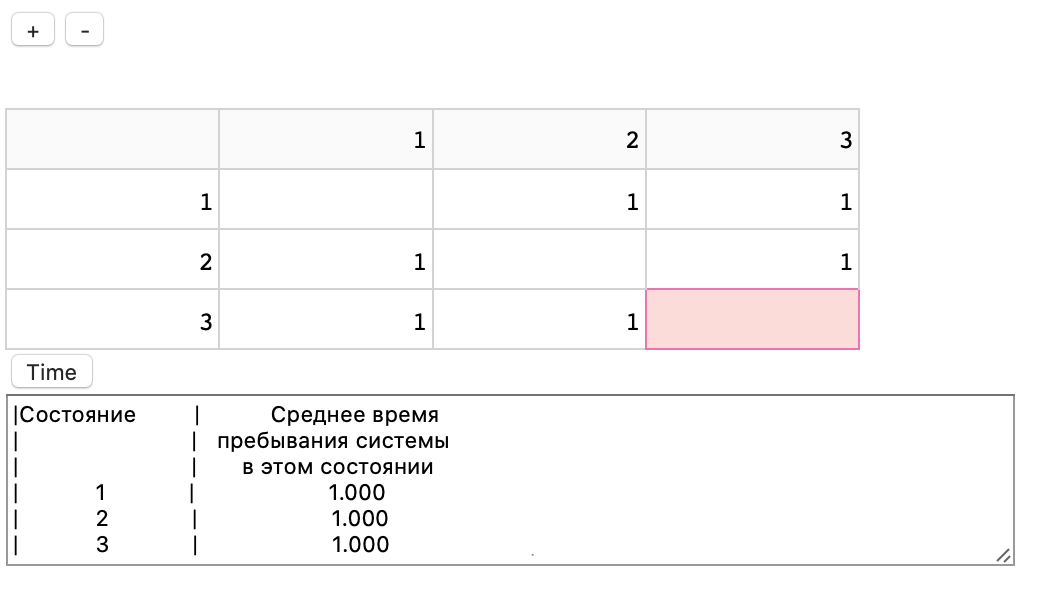
\includegraphics[scale=1]{1}
\end{figure}

\begin{figure}[H]
  \centering
  \caption{Пример 2. }
  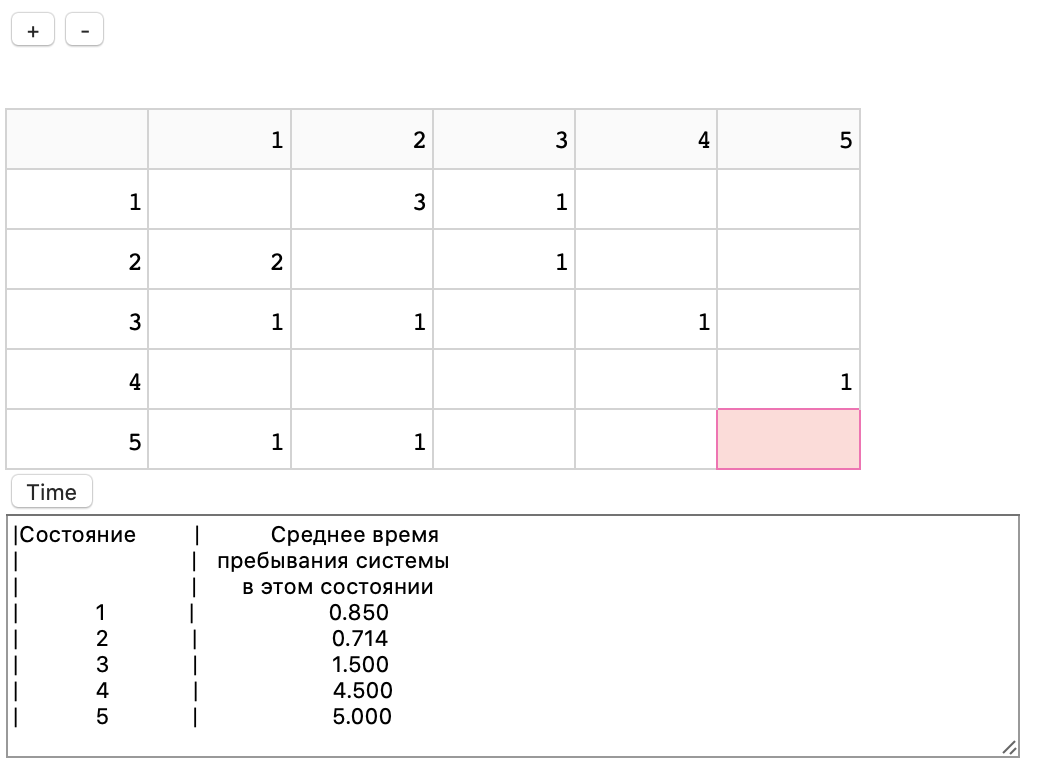
\includegraphics[scale=1]{2}
\end{figure}

\begin{figure}[H]
  \centering
  \caption{Пример 3. }
  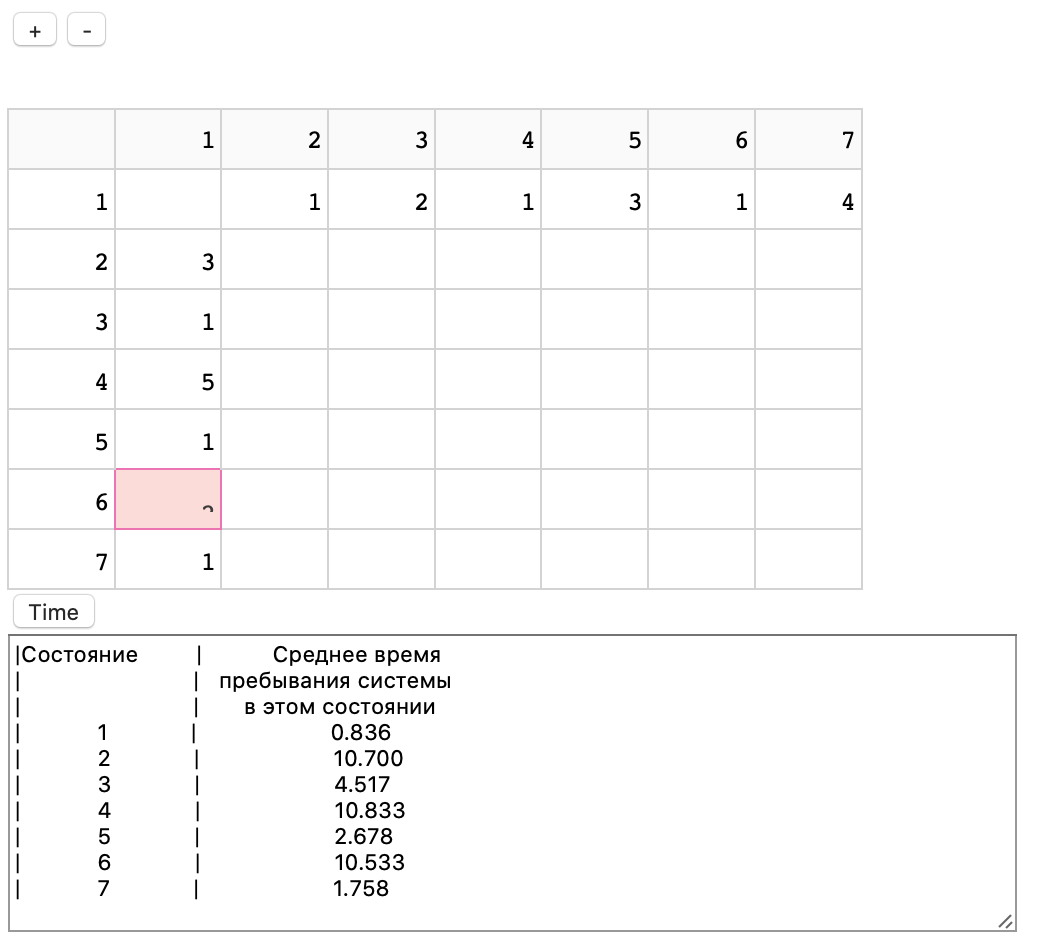
\includegraphics[scale=1]{3}
\end{figure}

\item \textbf{Вывод. }
\end{enumerate}
Была написана программа, которая для сложной системы S, имеющей не более 10 состояний определяет среднее и среднее относительное время нахождения системы в предельных состояниях, то есть при установившемся режиме работы. 

\end{document}